\documentclass[../../eatbrain.tex]{subfile}
Le pagine Releaes e Podcasts sono praticamente identiche e portano gli stessi difetti nell'\textbf{How} descritti dalla pagina \hyperref[sec-artists]{\texttt{Artists}}. \\
L'unica differenza, come citato nella sezione \hyperref[convenzioni]{\texttt{Rispetto Delle Convenzioni}}, sta nei link cliccabili: per accedere alla specifica delle tracce bisogna cliccare sul testo e non sulle immagini. \\
Una particolare precisazione va fatta sull'asse \textbf{When}: sebbene questo sia facoltativo nelle pagine interne, il particolare contenuto della pagina ne richiederebbe la specificazione. Le varie tracce presenti sono si disposte in ordine cronologico, ma senza conoscenza preliminare non è possibile capirlo: non esiste da nessuna parte una data di rilascio del contenuto musicale e neanche nelle pagine interne viene citata questa informazione. Sebbene l'ordine cronologico può essere intuito questa sottigliezza può peggiorare la valutazione dell'utente. \\
\begin{figure}[h]
	\centering
	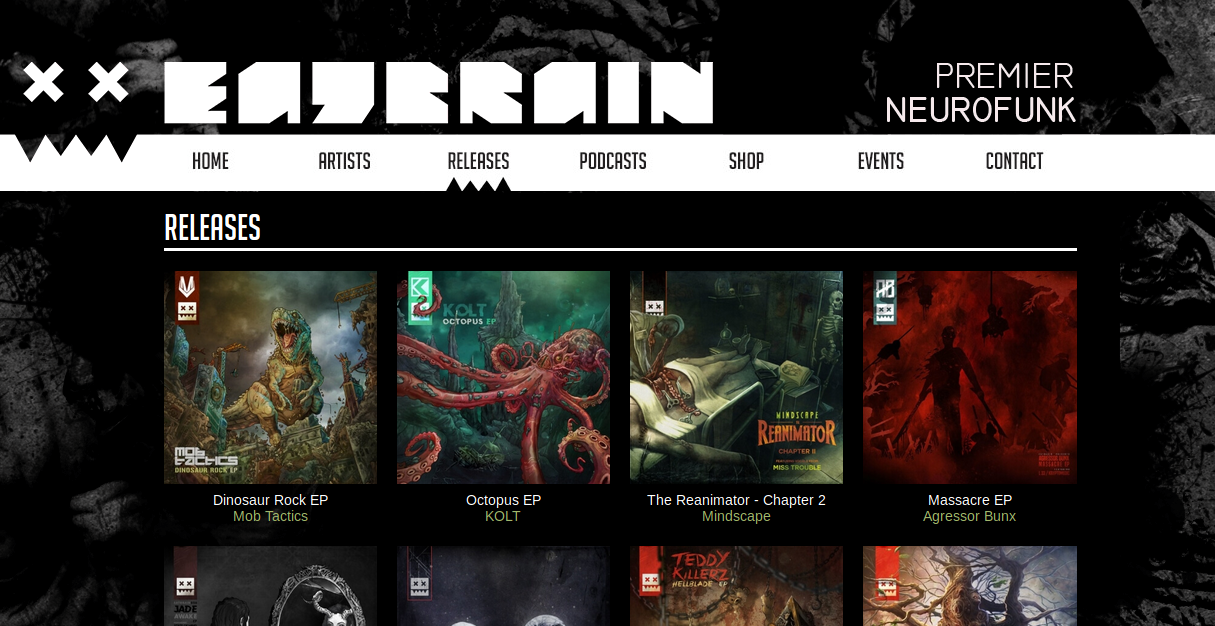
\includegraphics[width=11.5cm]{immagini/releases}
	\caption{Snapshot della pagina Releases}
	\label{img-releases}
\end{figure}
\newpage